
%\documentclass[nototal]{beamer}
\documentclass[nototal,handout]{beamer}

% This file is a solution template for:

% - Talk at a conference/colloquium.
% - Talk length is about 20min.
% - Style is ornate.


%
% In principle, this file can be redistributed and/or modified under
% the terms of the GNU Public License, version 2.
%
% However, this file is supposed to be a template to be modified
% for your own needs. For this reason, if you use this file as a
% template and not specifically distribute it as part of a another
% package/program, I grant the extra permission to freely copy and
% modify this file as you see fit and even to delete this copyright
% notice. 


\mode<presentation>
{
  \usetheme{Madrid}
  %\usetheme{Boadilla}
  % or ...

  \setbeamercovered{transparent}
  % or whatever (possibly just delete it)
}


\usepackage[english]{babel}
% or whatever

\usepackage[latin1]{inputenc}
% or whatever

\usepackage{times}
\usepackage[T1]{fontenc}
% Or whatever. Note that the encoding and the font should match. If T1
% does not look nice, try deleting the line with the fontenc.
\usepackage{graphicx} %sjr added
\graphicspath{{figures/}}
\usepackage{hyperref}
\author{\textsc{Sergio Rey}}
\institute[ASU]{\textbf{GPH 483/598}\\\textbf{Geographic Information
Analysis}\\School of Geographical Sciences\\Arizona State University\\Spring
2010}
\title[GPH 483/598]{Point Pattern Analysis: Processes (2)}
\subtitle{}
\date[Point Pattern Processes (2)]{}



% If you have a file called "university-logo-filename.xxx", where xxx
% is a graphic format that can be processed by latex or pdflatex,
% resp., then you can add a logo as follows:

% \pgfdeclareimage[height=0.5cm]{university-logo}{university-logo-filename}
% \logo{\pgfuseimage{university-logo}}



% Delete this, if you do not want the table of contents to pop up at
% the beginning of each subsection:
\AtBeginSubsection[]
{
  \begin{frame}<beamer>
    \frametitle{Outline}
    \tableofcontents[currentsection,currentsubsection]
  \end{frame}
}


% If you wish to uncover everything in a step-wise fashion, uncomment
% the following command: 

%\beamerdefaultoverlayspecification{<+->}


\begin{document}

\begin{frame}
  \titlepage
\end{frame}

\begin{frame}
  \frametitle{Outline}
  \tableofcontents
  % You might wish to add the option [pausesections]
\end{frame}


% Structuring a talk is a difficult task and the following structure
% may not be suitable. Here are some rules that apply for this
% solution: 

% - Exactly two or three sections (other than the summary).
% - At *most* three subsections per section.
% - Talk about 30s to 2min per frame. So there should be between about
%   15 and 30 frames, all told.

% - A conference audience is likely to know very little of what you
%   are going to talk about. So *simplify*!
% - In a 20min talk, getting the main ideas across is hard
%   enough. Leave out details, even if it means being less precise than
%   you think necessary.
% - If you omit details that are vital to the proof/implementation,
%   just say so once. Everybody will be happy with that.

\section{Clustered Patterns}

\begin{frame}[<+->]
  \frametitle{Clustered Pattern}
  \begin{block}{More Grouped than CSR}
    \begin{itemize}
      \item some higher densities, aggregated
	\item many points at shorter distances
    \end{itemize}
   \end{block}
   \begin{block}{Overdispersion}
     \begin{itemize}
      \item variance > mean
      \item greater variation in densities than CSR
     \end{itemize}
   \end{block}
 \end{frame}
\begin{frame}[<+->]
  \frametitle{Sources of Clustering}
  \begin{block}{Contagion}
    \begin{itemize}
      \item presence of events at $x$ affects probability of event at $y$
      \item correlated point processes
    \end{itemize}
   \end{block}
   \begin{block}{Heterogeneity}
     \begin{itemize}
      \item intensity $\lambda(s)$ varies with $s$
       \item heterogeneous Poisson point process
     \end{itemize}
   \end{block}

 \end{frame}

 \begin{frame}[<+->]
   \frametitle{Contagious Distributions}
   \begin{block}{Two stages}
     \begin{itemize}
       \item point pattern for parents
       \item point pattern for offspring centered on parent locations
       \item parents may or may not be included
     \end{itemize}
    \end{block}

    \begin{block}{Examples}
      \begin{itemize}
	\item Poisson cluster process (Neyman-Scott)
	\item Matern cluster process
      \end{itemize}
    \end{block}
  \end{frame}

 \begin{frame}[<+->]
   \frametitle{Poisson Cluster Process}
   \begin{block}{Parent Events}
     \begin{itemize}
       \item Poisson process with intensity $\lambda$
     \end{itemize}
    \end{block}

    \begin{block}{Number of Offspring Events $S$}
      \begin{itemize}
	\item identical distribution for each parent
	\item $E[S] = \mu$
      \end{itemize}
     \end{block}

    \begin{block}{Location of Offspring Events}
      \begin{itemize}
	\item independent and identically distributed
	\item following a bivariate density $h$ 
      \end{itemize}
     \end{block}
  \end{frame}

\begin{frame}
  \frametitle{Example}
  \begin{block}{Parent Process Poisson}
    \begin{itemize}
      \item homogeneous, intensity $\lambda$ constant
    \end{itemize}
   \end{block}
 \begin{block}{Child Process }
    \begin{itemize}
      \item uniform points in circle centered on parent
      \item fixed number of points in circle centered on parent
      \item points outside window eliminated
    \end{itemize}
   \end{block}
\end{frame}
\subsection{Neyman Scott}
\begin{frame}
	\frametitle{Neyman Scott $\lambda=10, S=5$}
 \begin{figure}[ht]
  \begin{minipage}[b]{0.4\linewidth}
  \centering
  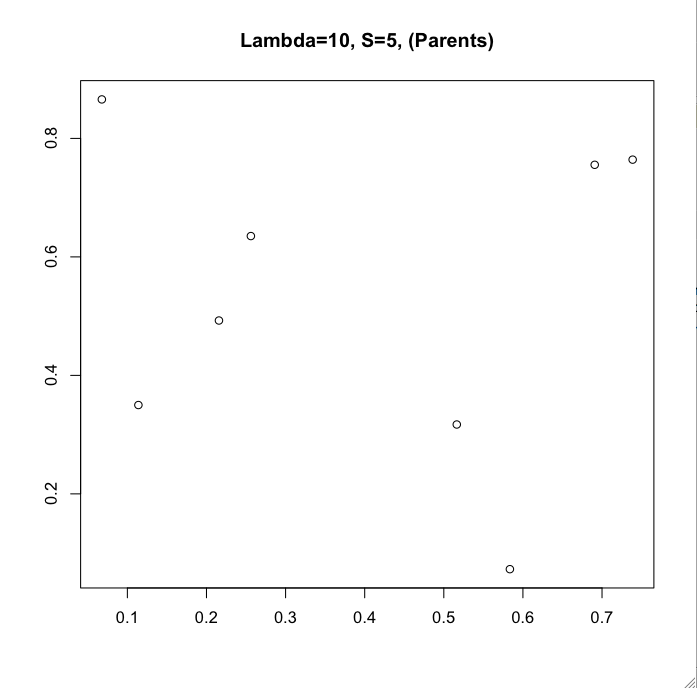
\includegraphics[scale=0.20]{ns105p.png}
  \end{minipage}
  \begin{minipage}[b]{0.4\linewidth}
  \centering
  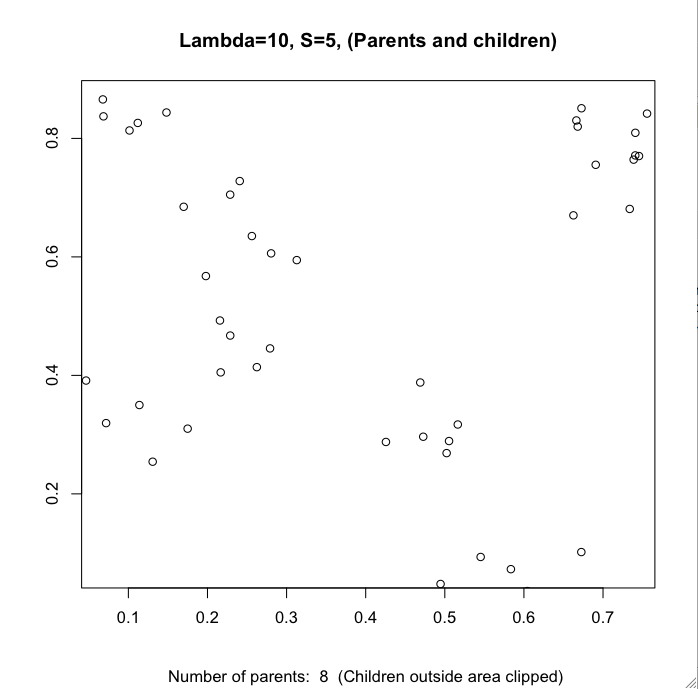
\includegraphics[scale=0.20]{ns105c.png}
  \end{minipage}

  \end{figure}
 \end{frame} 


\begin{frame}
	\frametitle{Neyman Scott $\lambda=5, S=10$}
 \begin{figure}[ht]
  \begin{minipage}[b]{0.4\linewidth}
  \centering
  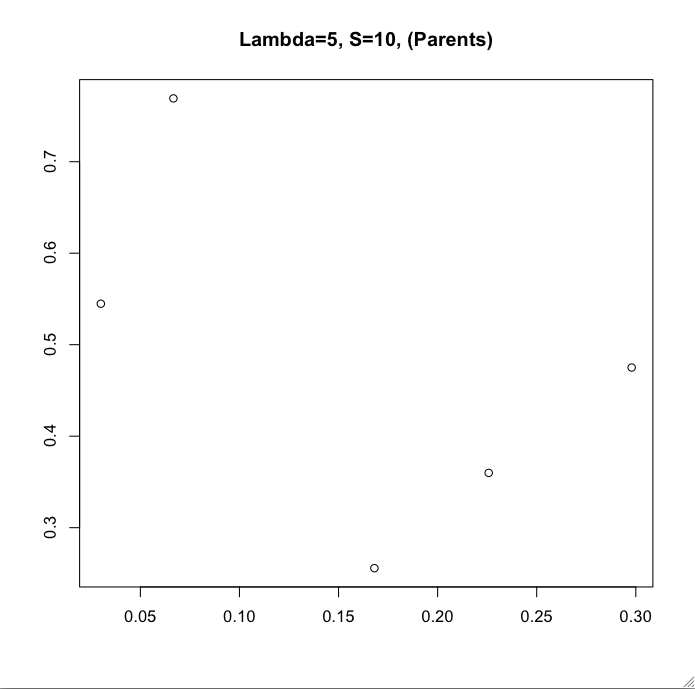
\includegraphics[scale=0.20]{ns510p.png}
  \end{minipage}
  \begin{minipage}[b]{0.4\linewidth}
  \centering
  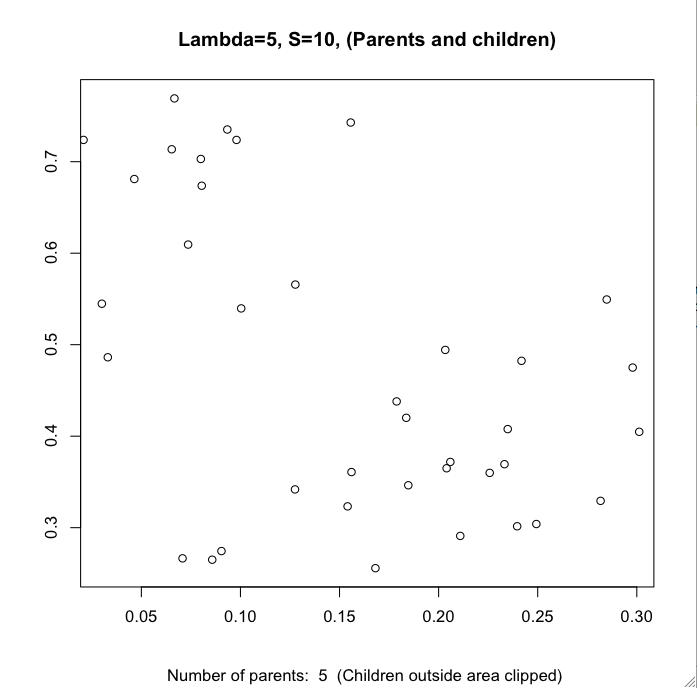
\includegraphics[scale=0.20]{ns510c.png}
  \end{minipage}

  \end{figure}
 \end{frame} 
 \subsection{Inhomogeneous Poisson Process}
\begin{frame}[<+->]
  \frametitle{Inhomogeneous Poisson Process}
  \begin{block}{Implications}
    \begin{itemize}
      \item Apparent clusters can occur solely due to heterogeneities in the intensity
	function $\lambda(s)$.
      \item Individual event locations still remain independent of one
	another.
      \item Process is not stationary due to intensity heterogeneity
    \end{itemize}
   \end{block}
   \begin{block}{HPP vs. IPP}
       HPP is a special case of IPP with a constant intensity
   \end{block}
 \end{frame}

\begin{frame}[<+->]
  \frametitle{CSR vs. Constant Risk Hypotheses}
  \begin{block}{CSR}
    \begin{itemize}
      \item Intensity is spatially constant 
      \item Population at risk assumed spatially uniform 
      \item Useful null hypothesis if these conditions are met
    \end{itemize}
   \end{block}
  \begin{block}{Constant Risk Hypothesis}

    \begin{itemize}
      \item Population density variable
      \item Individual risk constant
      \item Expected number of events should vary with population density
      \item Clusters due to deviation from CSR
      \item Clusters due to deviation from CSR and Constant Risk
    \end{itemize}

  \end{block}
 \end{frame}


 \begin{frame}
   \frametitle{Inhomogeneous Poisson Process}
   \begin{block}{Non-Stationary}
     \begin{itemize}
       \item spatially varying intensity $\lambda(s)$
       \item mean is $\int_A \lambda(s) ds$
       \item an integral of the location-specific intensities over the region
     \end{itemize}
    \end{block}
    \begin{block}{Properties}
      \begin{itemize}
	\item $N(A) \sim Poi(\int_A \lambda(s) ds$
	\item $N(A)=n, \ n$ events independent sample with pdf proportional to
	  $\lambda(s)$
      \end{itemize}
     \end{block}
  \end{frame}
  \begin{frame}
    \frametitle{Sources of Variability}
    \begin{block}{Deterministic}
      \begin{itemize}
	\item function for variability of $\lambda(s)$
	\item introduce covariates: $\lambda(s) = f(z)$
      \end{itemize}
     \end{block}
   \begin{block}{Stochastic}
      \begin{itemize}
	\item doubly stochastic process
	\item distribution for $\lambda(s) \sim \Lambda(s)$
      \end{itemize}
     \end{block}
\end{frame}

\begin{frame}
  \frametitle{Examples}
  \begin{block}{Intensity Varies with a Covariate}
    \begin{itemize}
      \item trend surface
      \item $\lambda(s) = exp(\alpha + \beta s)$
    \end{itemize}
  \end{block}
  \begin{block}{Intensity Varies with Distance to Focus}
    \begin{itemize}
      \item $\lambda(s) = \lambda 0(s). f( || s-s_0||, \theta)$
    \end{itemize}
  \end{block}
\end{frame}

\begin{frame}
  \frametitle{Inhomogeneous Poisson Process: $\lambda(x,y)=100*exp(-3x)$}
 \begin{figure}[ht]
  \centering
  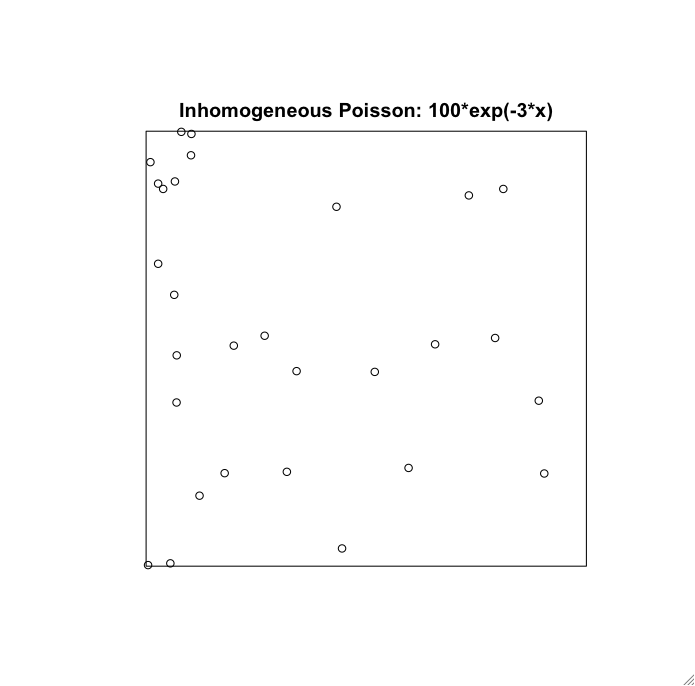
\includegraphics[scale=0.30]{ihpne.png}
  \end{figure}
 \end{frame} 

\begin{frame}
  \frametitle{Inhomogeneous Poisson Process: $\lambda(x,y)=100*exp(-3x)$}
 \begin{figure}[ht]
  \centering
  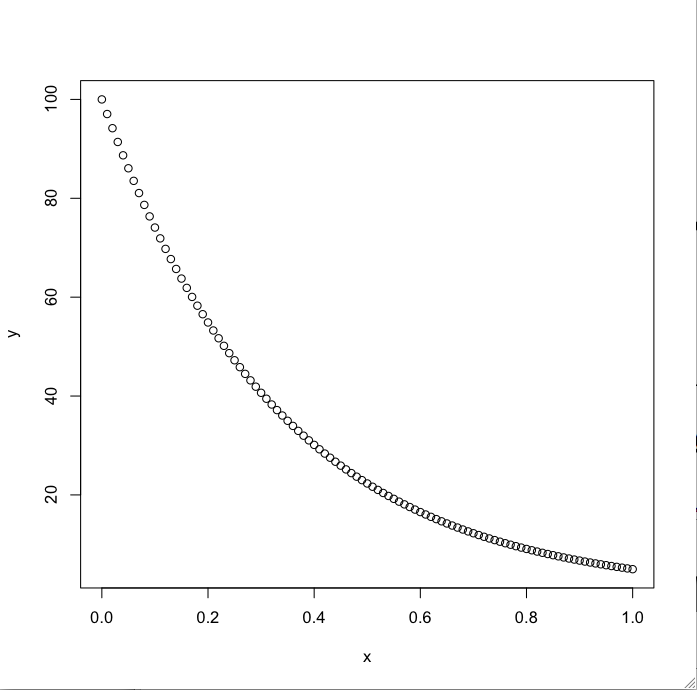
\includegraphics[scale=0.30]{ihpnef.png}
  \end{figure}
 \end{frame} 


\begin{frame}
  \frametitle{Inhomogeneous Poisson Process: $\lambda(x,y)=100*(x+y)$}
 \begin{figure}[ht]
  \centering
  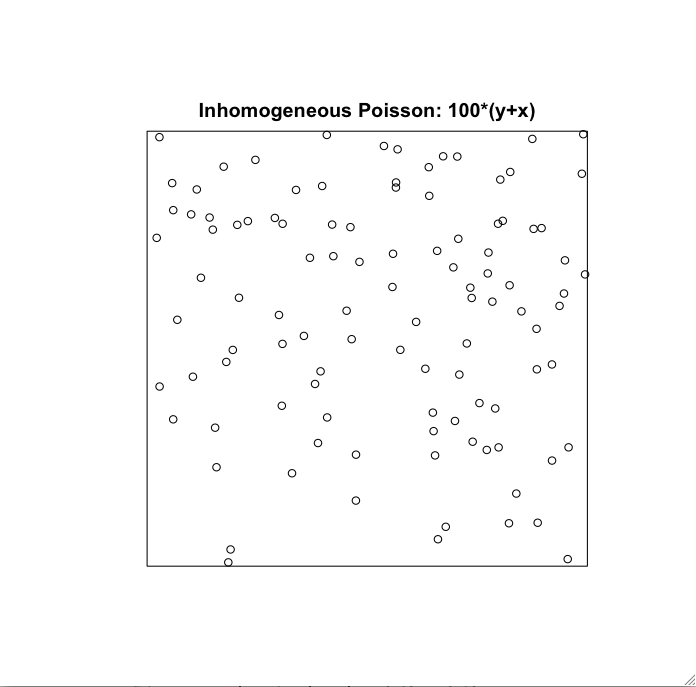
\includegraphics[scale=0.30]{ihpxy.png}
  \end{figure}
 \end{frame} 

\begin{frame}
    \frametitle{Thinning}
    \begin{block}{From Homogeneous to Heterogeneous}
      \begin{itemize}
	\item remove points
      \end{itemize}
    \end{block}

    \begin{block}{Types}
      \begin{itemize}
	\item $p$-thinning: constant probability
	\item $p(s)$-thinning: probability varies with $s$
	\item $\Pi$-thinning: thinning function is random
      \end{itemize}
    \end{block}
\end{frame}

\begin{frame}
  \frametitle{Simulation}
  \begin{block}{Start with homogeneous Poisson}
    \begin{itemize}
      \item $\lambda = max [ \alpha(s) ] $
    \end{itemize}
   \end{block}
 \begin{block}{Apply $p(s)$ Thinning}
	\begin{itemize}
	  \item keep points with probability $p(s)$
	  \item $p(s) = \alpha(s) /  \lambda$
	  \item e.g., keep if generated uniform random number < $p(s)$
	\end{itemize}
   \end{block}
\end{frame}

\begin{frame}
  \frametitle{Cox Process}
  \begin{block}{Doubly Stochastic Process}
    \begin{itemize}
      \item $\Lambda(s)$ is stochastic process over $A$
      \item events inhomogeneous Poisson process with $\lambda(s) =
	\Lambda(s)$ (a realization)
    \end{itemize}
   \end{block}
 \begin{block}{Log-Gaussian Process}
    \begin{itemize}
      \item $\Lambda(s)= exp[Z(s)]$ with $Z(s) \sim N(\mu, \sigma^w)$
      \item $E[\lambda] = exp(\mu + 0.5 \sigma^2)$
    \end{itemize}
   \end{block}
\end{frame}


\begin{frame}
	\frametitle{Cox process}
 \begin{figure}[ht]
  \centering
  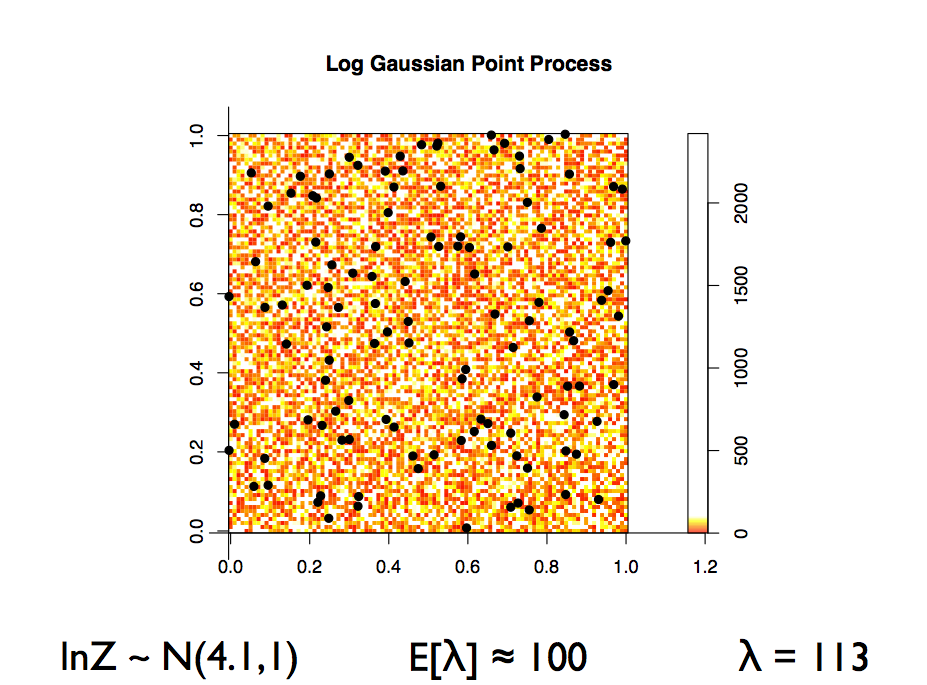
\includegraphics[scale=0.20]{cox.png}
  \end{figure}
 \end{frame} 



\begin{frame}
  \frametitle{Identification}
  \begin{block}{Inverse problem}
    \begin{itemize}
      \item identify process from pattern
    \end{itemize}
   \end{block}
 \begin{block}{True Contagion - Apparent Contagion}
    \begin{itemize}
      \item impossible to distinguish contagious process from heterogeneous process
    \end{itemize}
   \end{block}
\end{frame}

\begin{frame}
  \frametitle{Identification}
  \begin{block}{Bartlett Equivalence}
    \begin{itemize}
      \item Cox process (heterogeneity) and Poisson Cluster process
	(contagion) yield equivalent patterns
    \end{itemize}
   \end{block}
\begin{block}{Identification Strategies}
    \begin{itemize}
      \item repeated observation, covariates
      \item heterogeneous in same location, contagious not
    \end{itemize}
   \end{block}


 \end{frame}


\section{Regular Pattern}
\begin{frame}
  \frametitle{Regular Pattern}
  \begin{block}{Less Grouped than CSR}
    \begin{itemize}
      \item fewer high densities, empty space
      \item dispersed
      \item repulsion, competition
    \end{itemize}
   \end{block}
 \begin{block}{Underdispersion}
    \begin{itemize}
      \item variance < mean
      \item less variation in densities than CSR
    \end{itemize}
   \end{block}
\end{frame}


\begin{frame}
  \frametitle{Inhibition Process}
  \begin{block}{Minimum Permissible Distance}
    \begin{itemize}
      \item no two points closer than $\delta$
      \item packing intensity $\tau = \lambda \pi \delta^2/4$
    \end{itemize}
   \end{block}
  \begin{block}{Matern Process}
    \begin{itemize}
      \item I: thinned Poisson process using $\delta$
      \item II: sequential inhibition process,  generates points conditional on
	previous points and distance (denser than I)
    \end{itemize}
  \end{block}
 \end{frame}

 \subsection{Inhibition: Matern Processes}
\begin{frame}
	\frametitle{Matern I and II $\lambda=100$}
 \begin{figure}[ht]
  \begin{minipage}[b]{0.4\linewidth}
  \centering
  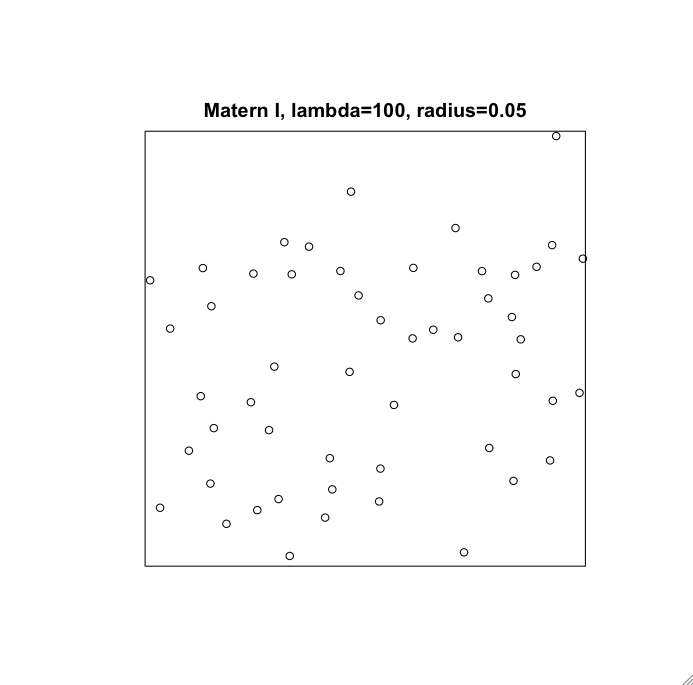
\includegraphics[scale=0.20]{matern1100.png}
  \end{minipage}
  \begin{minipage}[b]{0.4\linewidth}
  \centering
  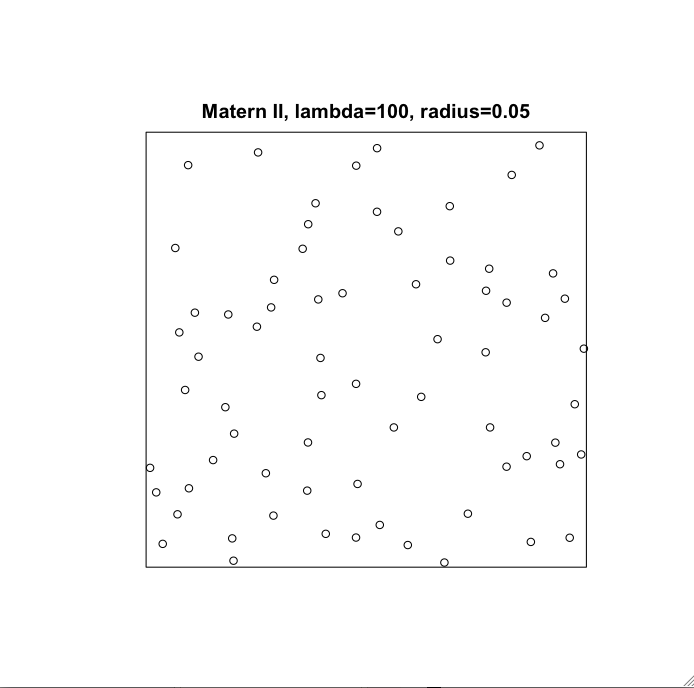
\includegraphics[scale=0.20]{maternII100.png}
  \end{minipage}

  \end{figure}
 \end{frame} 


\begin{frame}
	\frametitle{Matern I and II $\lambda=500$}
 \begin{figure}[ht]
  \begin{minipage}[b]{0.4\linewidth}
  \centering
  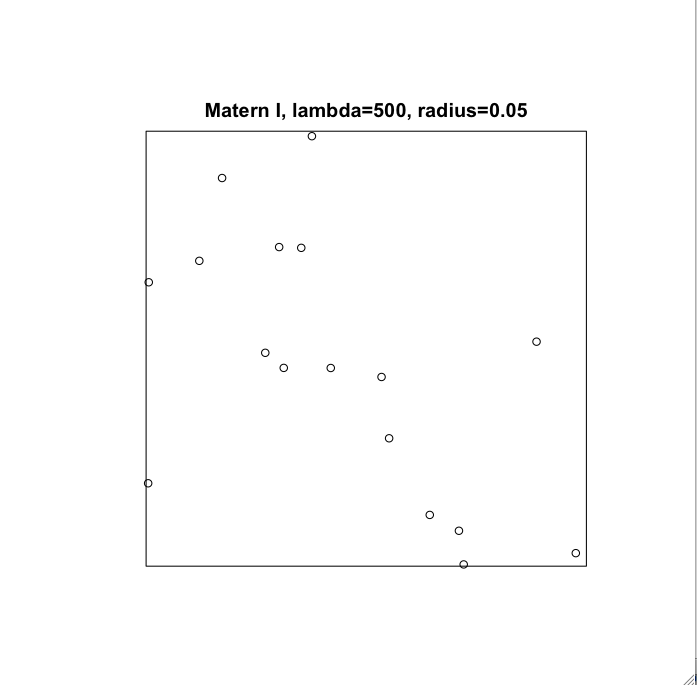
\includegraphics[scale=0.20]{maternI500.png}
  \end{minipage}
  \begin{minipage}[b]{0.4\linewidth}
  \centering
  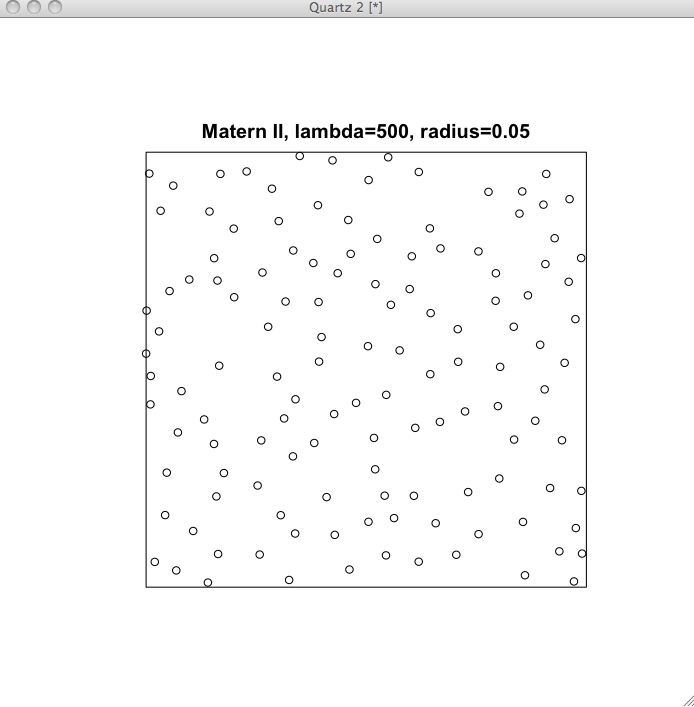
\includegraphics[scale=0.20]{maternII500.png}
  \end{minipage}

  \end{figure}
 \end{frame} 

 \subsection{Markov Point Processes}

 \begin{frame}
   \frametitle{Markov Point Processes}
   \begin{block}{Allow for Interaction}
     \begin{itemize}
       \item neighbors $||x - y || < \delta $, range of process
       \item likelihood relative to Poisson with $\lambda=1$
       \item $f(x) = exp(-|A|)$
     \end{itemize}
    \end{block}
\begin{block}{Strauss Process}
     \begin{itemize}
       \item $f(x) = \alpha \beta^n \gamma^s$
       \item $\beta$ intensity, $n$ number of points
       \item $\gamma$ interactions, $\gamma < 1$ is inhibition, $s$ pairs
     \end{itemize}
    \end{block}
  \end{frame}

  \begin{frame}
    \frametitle{Interaction Processes}
    \begin{block}{Pairwise Interaction Point Processes}
      \begin{itemize}
	\item $f(x) = \alpha \beta^n \prod_i \prod_{j\ne i} h(||x_i -
	  x_j||)$
	\item $h=0$ for $\delta > 0$
      \end{itemize}
     \end{block}
     \begin{block}{Area Interaction Point Processes}
       \begin{itemize}
	 \item $f(x) = \alpha \beta^n \alpha^{-A (X,\delta)}$
	 \item $\delta = 1:$ Poisson
	 \item $\delta < 1:$ inhibition
	 \item $\delta > 1:$ aggregated
       \end{itemize}
     \end{block}
   \end{frame}

\end{document}
